\section{Evaluation}
\label{sec:eval}

We evaluate RCuckoo by directly comparing its performance in terms of
throughput and latency against representative state-of-the-art
disaggregated key/value stores and find that RCuckoo outperforms them
all in terms of throughput while delivering competitive insert
latencies.  Using fault injection, we show that our distributed
approach to client failure detection and recovery enables RCuckoo to
sustain high throughput even though 100s of clients are failing per
second.  Finally, we justify our design decisions through a series of
micro-benchmarks. Specifically, we quantify the benefit RCuckoo
extracts from its locality enhancement and speculative search strategy
and conduct sensitivity analyses of our choice of locality parameter,
covering read threshold, and index-table entry size.

\section{Implementation}

Our implementation of RCukcoo consists of a of 8.7k C++
implementation and a 12k line Python implementation which
simulates RDMA. Both implementations will be made available
on Github.  All results reported in Section~\ref{sec:eval}
are from the C++ implementation. At the time of writing only
the python implementation includes support for delete
operations, and extent entries. As such all C++ results are
for inserts, reads, updates and inlined table operations.
RCuckoo is designed for ConnectX-5 NICs. It uses OFED-4.9
which supports experimental verbs for atomic masked CAS and
device mapped memory. 


\begin{figure*}[ht]
    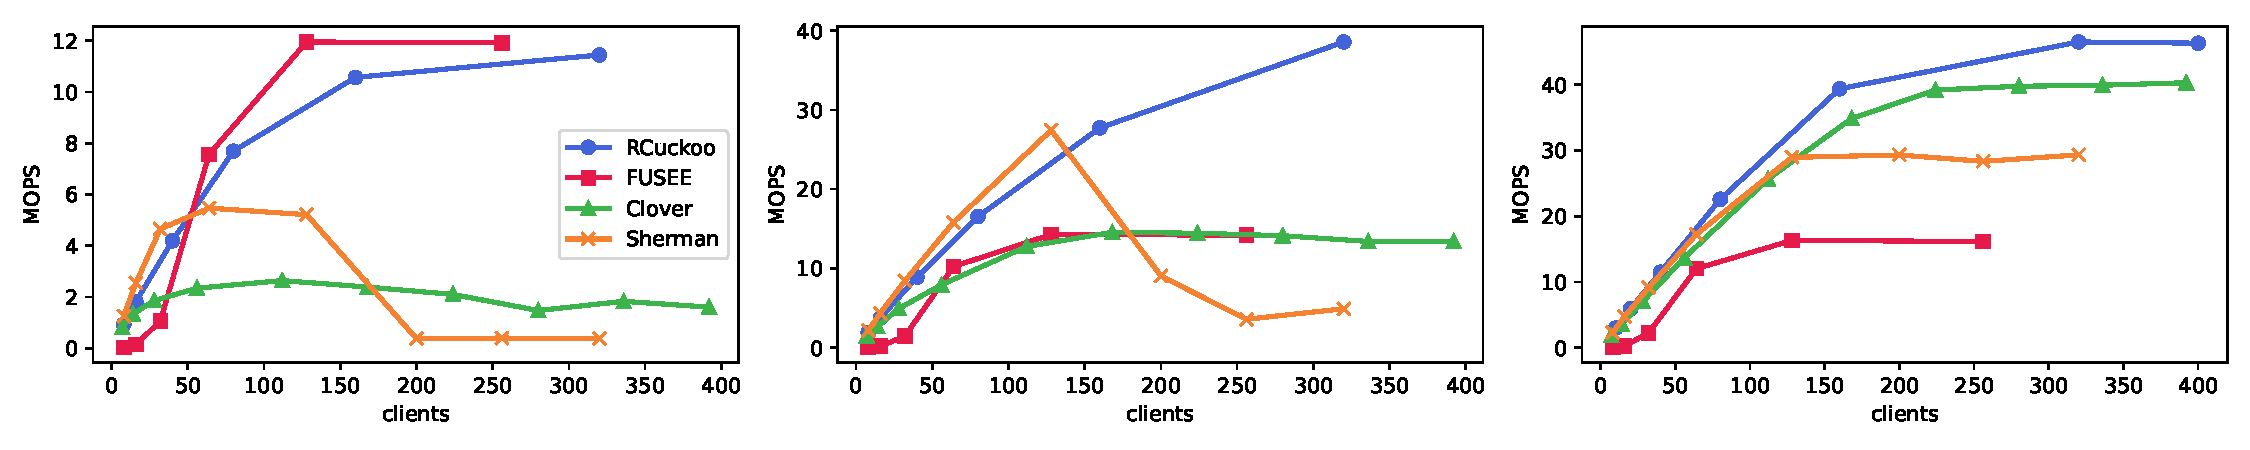
\includegraphics[width=0.99\linewidth]{fig/hero_ycsb_throughput.pdf}

    \caption{Throughput as a function of the number of clients for three different workloads (Zipf $\theta$=0.99): \textbf{(a)} YCSB-A 50\%
    read 50\% update, \textbf{(b)} YCSB-B 95\% read 5\% update and \textbf{(c)}
    YCSB-C 100\% read.}
    \label{fig:ycsb_throughput}
 \end{figure*}


\subsection{Testbed}

We conduct our evaluation on an 11-node cluster of dual-socket Intel
machines. Each CPU is an Intel Xeon E5-2650 clocked at
2.20~GHz. Each machine has 256~GB of RAM with 128~GB per NUMA
node. All machines have a single dual-socket ConnectX-5 attached to a
100-Gbps Mellanox Onyx switch. In our RCuckoo experiments we use one
sever as the memory server and the rest a client machines
spreading threads evenly across machines.

%\subsection{Comparison systems}

We compare RCuckoo against three recent RDMA key-value stores with
different designs, FUSEE~\cite{fusee}, Clover~\cite{clover}, and
Sherman~\cite{sherman}.  While none have the exact same assumptions or
feature set as RCuckoo, each represents an apt comparison point for
different aspects.  To avoid biasing our evaluation, we use the same
workloads (YCSB) as the previous efforts.
%
%We directly compare RCuckoo against three disaggregated
%key-value stores  Each system has distinct design
%tradeoffs. 
%%
%%
%%

\textbf{FUSEE} is a fully disaggregated key/value store that
represents the closest available comparison point to RCuckoo.  While
both employ only 1-sided RDMA operations, FUSEE eschews locking in
favor of optimistic insertions.  FUSEE clients use CAS operations
to manage fixed, 64-bit index table entries that contain pointers to
values stores in extents.  Due to its reliance on CAS operations, FUSEE is unable to support inlined storage of small
values like RCuckoo, forcing all reads to require two round trips.
%Fusee is the closest comparison we have to illustrate
%the tradeoffs between locks and optimistic concurrency.
%is a key-value store designed for full
%disaggregation~\cite{fusee}.  It is built on top of RACE~\cite{race}
Unlike RCuckoo, FUSEE is designed to support replication.  To remove the overhead of replication, 
%While RACE represents a more direct comparison to RCuckoo, no open
%source implementation of RACE is available.  Instead,
we deploy FUSEE with a single memory node.
%FUSEE/RACE hashing uses fixed-sized 64-bit index entries
%to in order to employ RDMA compare-and-swap operations for updates. As
%such, RACE-based systems cannot store key-value pairs in the index
%table itself and require a second round trip even for reads of small values.
%on reads to recover
%extent entries which contain full key value pairs.

\textbf{Clover} is only partially disaggregated---it requires a
metadata server to manage its index structure---but can deliver higher
read performance than FUSEE on read-only workloads.  Clover is
designed to leverage remote persistent memory and implements both
reads and updates using one-sided RDMA operations.  Moreover, unlike
FUSEE---and similar to RCuckoo---Clover reads are self verifying.
%Clover uses index caching to optimize reads.  When re-reading key-value
%entires clover can as it directly
%reads the entry without negotiating with the index.
In contrast to prior Clover comparisons~\cite{fusee} that force
clients to consult the metadata server on each read, we allow Clover
to take advantage of its client caching to achieve maximum performance
on read-heavy workloads.

%% Clover is a partially disaggregated system which uses
%% two-sided RDMA operations to modify the index and one-sided
%% operations for updates, deletes, and reads.

%% Sherman a disaggregated B-Tree and the only system at the
%% time of writing which uses locks and not optimistic
%% concurrency to guard its index. Our performance comparison
%% with Sherman is not apples to apples. Sherman maintains
%% ordered key-value pairs for range queries and thus has
%% higher overheads on updates than the other systems.

\textbf{Sherman} is the highest-throughput distributed key/value
storage system of which we are aware that employs locks.  Sherman
maintains a B-tree that spans multiple servers and supports range
queries, a feature none of the other systems---RCuckoo
included---provide.
%is a B-tree designed for remote memory~\cite{sherman}.
%and high write
%throughput.
%Unlike Clover and FUSEE which employ optimistic consistency control,
%Sherman uses locks to guard updates similar to RCuckoo.
On the other
hand, Sherman clusters are not fully disaggregated: each node in a
cluster is a peer with many CPU cores and a single memory core
that is responsible for servicing allocation RPC calls from clients.
%Unlike the other systems
%Sherman is cluster based, and does not support a having
%isolated memory machines.
%All machines are equal nodes in a
%cluster and run both a memory controller and client threads.
As such, Sherman does not encounter the same bandwidth bottlenecks as
the other systems because requests are partitioned across all
machines in the cluster.
%However, it assumes that collocated clients can resolve lock
%contention locally and clients collocated with their segment
%of the B-Tree can perform local operations. These
%assumptions enable Sherman to have high performance under
%contention even though it uses locks and manages a more
%complex data structure than the unordered key-value stores.
%While Sherman does not meet the fully disaggregated model it
%does provide a good comparison for RCuckoo as it is the only
%other system to use locks in remote memory.


% \subsubsection{Clover}
% \todo{insert a short clover description}

\begin{figure*}[ht]
    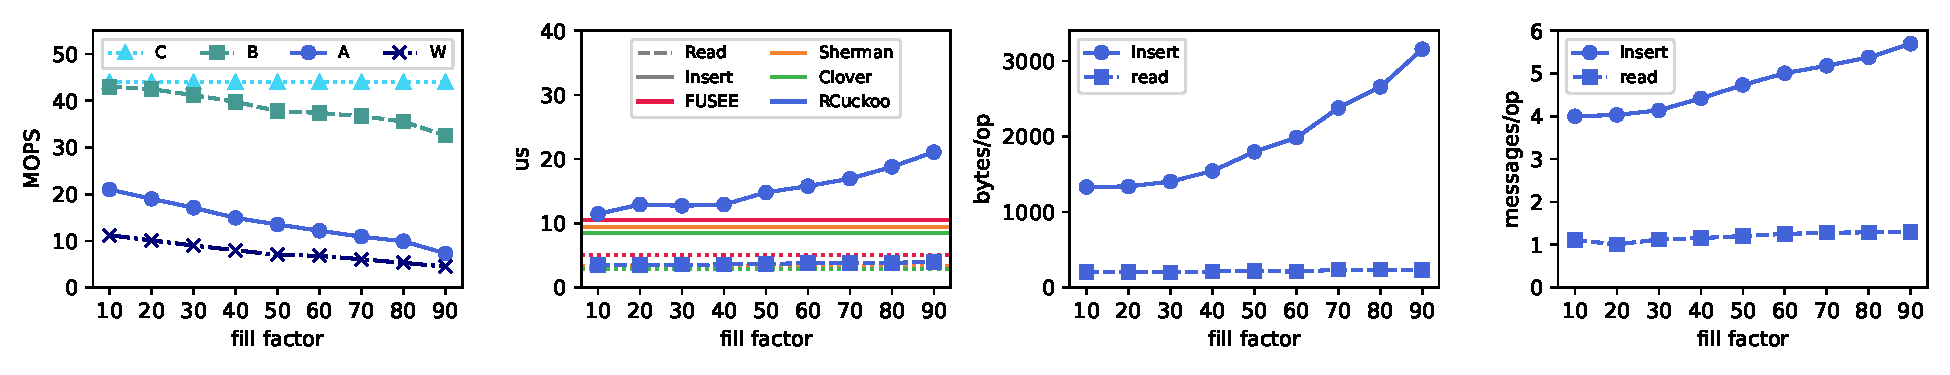
\includegraphics[width=0.99\linewidth]{fig/hero_ycsb_fill.pdf}

    \caption{Performance as a
    function of fill factor. \textbf{(a)} Throughput for four different YCSB insert workloads, \textbf{(b)}
    median operation latency, \textbf{(c)} mean operation size, and \textbf{(d)}
    mean RDMA message count per operation under YCSB-A.}

    \label{fig:ycsb_fill}
\end{figure*}

% \begin{figure}[ht]
%     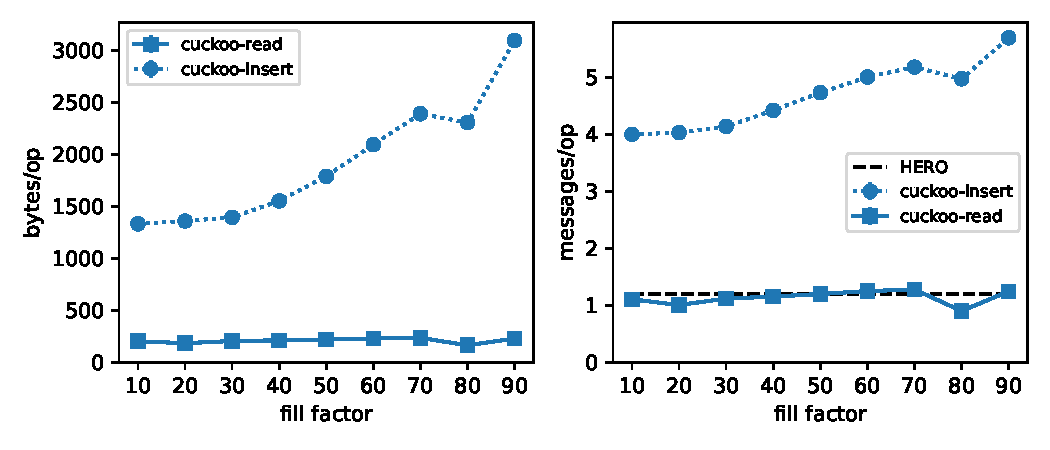
\includegraphics[width=0.99\linewidth]{fig/hero_ycsb_fill_ops_bw.pdf}
%     \caption{YCSB-A workload messages and bandwidth per operation as a function of fill factor}
%     \label{fig:ycsb_fill_ops_bw}
% \end{figure}



\subsection{Performance}

We start by considering the classical YCSB workloads which employ
varying mixes of read and update operations before turning to the more
complex insert operation.  RCuckoo delivers the highest performance
across all settings, while the others each shine on different
mixes.
\todo{What is the row/read size?  How close are we to line rate?}

\textbf{YCSB:}
Figure~\ref{fig:ycsb_throughput} shows throughput in terms of
operations per second for RCuckoo, FUSEE, Sherman, and Clover on
three different YCSB workloads with a Zipf(0.99) distribution. YCSB-A
is a 50\% read 50\% update, YCSB-B is 95\% read and 5\% update, and
YCSB-C is 100\% read.  In each experiment a variable number of clients
insert 90-M entries containing 32-bit keys and 32-bit values into a
100-M-entry hash table.


On YCSB-A RCuckoo begins to surpass FUSEE after about 125 clients.  FUSEE's maximum performance is gated by its requirement for an additional round trip per operation (to
retrieve the extent). Sherman keeps pace until about 5 MOPS at which
point it suffers from lock contention due to its B-Tree structure.
(Sherman and RCuckoo perform similarly for uniform workloads where
lock contention is less of an issue.).  Clover performs the worst
under write-heavy workloads due to its inability to effectively leverage
client-side caching of a constantly changing index structure.

On read-mostly and read-only workloads (YCSB-B and C)
RCuckoo extracts even further benefit over FUSEE from its ability to
complete read in a single round trip rather than two and gains
additional benefit by collapsing most reads into a single packet
(Section~\ref{sec:read_threshold}).  Sherman performs well on
read-mostly workloads as it can directly read from the B-Tree in a
single round trip without the need for pointer chasing, but it
continues to bottleneck on lock contention in YCSB-B due to hot
keys. While Sherman experiences no such bottleneck on YCSB-C its read
algorithm is more complex than RCuckoo's leading to lower top-end
performance. Clover performs similarly to FUSEE on YCSB-B, and is the
most competitive with RCuckoo in read-only scenario.  When it is able
to leverage its client index cache, Clover's reads are very similar to
RCuckoo in that they require only a single 1-sided RDMA read;  we
suspect that with tuning Clover's read-only performance
could be brought to par with RCuckoo.

\textbf{Inserts:}
%%
%By default YCSB-A,B,C use updates. RCuckoo's insert
%algorithm is it's most complex and bandwidth intensive
%component. In this section
Despite its complexity, RCuckoo's insert operation remains highly
performant.  To evaluate insert performance we modify YCSB to perform
inserts rather than updates.  Figure~\ref{fig:ycsb_fill} considers
RCuckoo's performance on workloads that exclusively use inserts (rather than
updates), for example in this instance YCSB-A is 50\% insert and 50\%
read. YCSB-W is write only, i.e. a 100\%-insert workload.  Inserts become
more expensive as the table fills, so we report insert performance as
a function of the table's fill factor.

Figure~\ref{fig:ycsb_fill}(a) shows the aggregate throughput
of 400 clients across four different workloads as a function
of the table's fill factor.  As the index table fills,
cuckoo paths become longer leading to increased contention
and additional bandwidth consumption from larger covering
reads. In each case (except YCSB-C) RCuckoo's performance
declines with fill factor. In the insert-only YCSB-W case
RCuckoo's performance drops from 11.5 to 4.5 MOPS.  As a
point of comparison, FUSEE's maximum insert-only performance
is 9.1 MOPS on our testbed, although it is independent of
fill factor.  While FUSEE out-performs RCuckoo at high fill
factors, we observe that an insert-only workload is uncommon
in practice~\cite{facebook-memcached}.

We plot operation latency, size, and message counts (in
terms of RDMA packets) as a function of fill factor in
Figure~\ref{fig:ycsb_fill}(b--d).  For comparison, we report
latency values of insert and read operations for the
comparison systems. These values were not collected under
load and represent best-case performance on our testbed.
Read latency is nearly identical for all systems save FUSEE,
as it requires an additional round trip.  Insert times vary:
Clover and Sherman use two-sided RDMA operations for insert
and both need to perform allocations and set up metadata for
the requesting client.  FUSEE is slightly slower, roughly
the same as RCuckoo's best case.  As the table fills,
however, cuckoo paths grow in length causing RCuckoo insert
operations to require additional round trips to find valid
cuckoo paths.  At maximum fill, insert operations take
roughly twice as long as in an empty table. This rising costs
is reflected by the increase in both bytes (Figure~\ref{fig:ycsb_fill}(c)) and messages (Figure~\ref{fig:ycsb_fill}(d)) per
operation.  RCuckoo reads, on the other hand, have roughly
the same cost and performance regardless of fill factor.


\begin{figure}[t]
    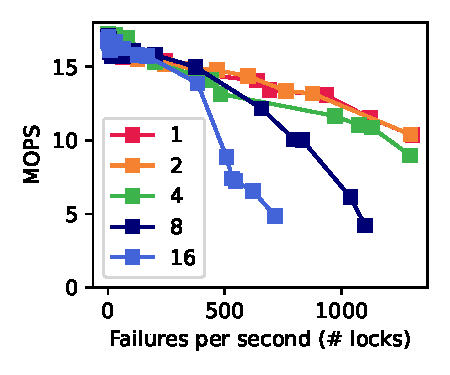
\includegraphics[width=0.99\linewidth]{fig/fault-rate.pdf}
    \caption{Throughput vs failure rate.}
    \label{fig:failure_throughput}
    \vskip -1em
\end{figure}

\subsection{Fault tolerance}

RCuckoo runs at nearly full throughput during realistic
failure scenarios and remains functional in the face of
hundreds of failures per second. When a client fails while
holding a lock the lock is stranded and requests for that
lock will block until after a client times out and reclaims
the lock.
%%
We emulate hundreds of client failures per second by
performing a partial insert operation which truncates the
batch of insert packets including lock releases. The table
entries are left in one of the inconsistent states listed in
Section~\ref{sec:table-repair} and locks are left set.


Figure~\ref{fig:failure_throughput} illustrates RCuckoo's
ability to operate at high throughput in the face of
failures. Lock granularity increases the probability that
multiple clients will block on the same failed lock. Larger
locks have little difference when failures are semi-frequent
and have a larger impact as hundred of failures occur per
second.  The performance impact of a few number of failures
per second is low which is ideal considering that failures
in RDMA clusters are relatively rare.  As a point of
reference, we observe that RCuckoo can still operate despite
thousands of failures per second while a server can only
establish approximately 1.4~K RDMA connections per second
using state of the art techniques~\cite{xrdma}.

\subsection{Microbenchmarks}

Having established RCuckoo's superiority over prior systems and
demonstrated its robustness to client failure, we now evaluate the
impact of particular design choices.

\subsubsection{Locality enhancement}

\begin{figure}[t]
    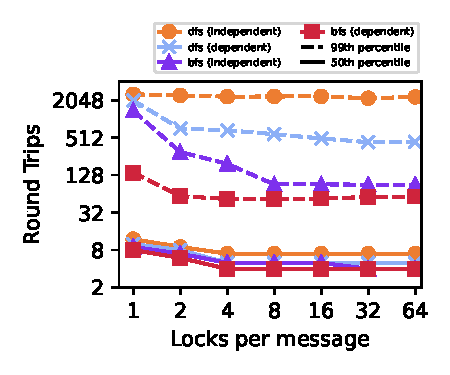
\includegraphics[width=0.99\linewidth]{fig/search_dependence.pdf}

    \caption{Round trips per insert operation with independent
    and dependent hashing.  (Note log-scale axes.)}

    \label{fig:search_dependence}
\end{figure}

%Hash dependence and search function choice have the highest
%impact on RCuckoo's performance. Dependent hashing reduces
%the probability locks are scattered throughout the table
%which enables RCuckoo to combine lock requests into a few
%masked CAS messages. Simultaneously search function choice
%dramatically affects the length of cuckoo paths.

Figure~\ref{fig:search_dependence} illustrates the dramatic benefit
RCuckoo extracts from its dependent hashing combined with a BFS
cuckoo-path search strategy.  To focus on longer cuckoo paths, we
pre-fill a 100-M entry table to 85\% and then report both the median
and 99th percentile number of round trips required to insert new
key/value pairs until the table is 95\% full as a function of lock
granularity.  While median performance is on the same order, the
99th-percentile insert takes an order of magnitude fewer round trips
with dependent hashing and BFS as opposed to independent hashing and
DFS as used in prior cuckoo hash
systems~\cite{cuckoo-improvements,pilaf,cuckoo}.  As before
(c.f. Figure~\ref{fig:cuckoo-problems}), performance is similar with
four or more locks per message.

%% We vary the number of locks per message to demonstrate the
%% effect of path length and show why masked cas plays an
%% important role in RCuckoo's performance. We measured both
%% the median, and 99th percentile round trips per request on a
%% table with 100M entries. We fill the table to 85\% and then
%% executed insert operations to 95\%.

%% DFS with no hash dependence has extremely poor performance
%% at it's tail, taking over 2K round trips to complete. Both
%% at it's median and 99th percentile it sees only small
%% benefits from setting multiple locks per request as the
%% locks are scattered throughout the table. DFS with
%% dependence has far lower tail latency, and improves the
%% number of locks which can be acquired per message, however
%% it still constructs long rather than minimum length paths.
%% BFS with dependence provides the best performance and gains
%% the most from setting more locks per request. At 64 locks
%% per request it has 7.5x lower round trips at it's 99th
%% percentile and 4 rather than 5 round trips on average. We
%% found that A* search provided the same minimal path length
%% as DFS with slightly better locality. It's performance
%% against BFS was only superior at fill factors above 95\% and
%% lower elsewhere due to a higher runtime cost on short paths.



% Hash function locality hash a major impact in RCuckoo's
% performance.  Acquiring locks can only be done in a few
% round trips when the locks are clustered together tightly in
% the lock table.  Furthermore, the search function used to
% determine the cuckoo path has a large impact on the locality
% of the locks necessary to lock the path. We evaluate
% dependent hashing and independent hashing as well as random
% and a* search. We measure the number of round trips required
% for each control as a function of the number of locks which
% can be acquired per round trip.

% Figure~\ref{fig:search_dependence} shows the performance
% improvements gained by both locality hashing and A* search.
% In this experiment the table is filled from 0 to 90\% full
% with a YCSB-w workload. We measure the 99th percentile of
% round trips for these workloads. Random search with
% independent hashing leads to a large number of round trips
% as locks are scattered throughout the table. RDMA masked CAS
% operation do little here to reduce the round trips as they
% can rarely acquire more than one lock in a round trip. With
% dependent hashing and random search RDMA CAS operation are
% almost sufficient to reduce round trips, however the absolute
% number of locks required per insert is high which leads to
% greater contention. A* search with dependent hashing has
% cuckoo paths that are both short, and clustered together.


\subsubsection{Speculative search}

\label{sec:search_success}
\begin{figure}[t]
    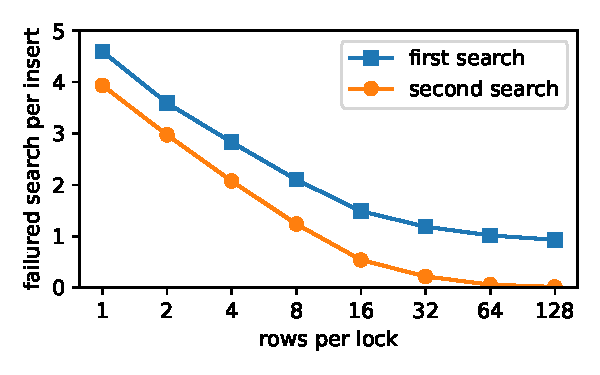
\includegraphics[width=0.99\linewidth]{fig/search_success_lock_size.pdf}
    \caption{Failure rate of search algorithms vs lock size under high contention}
    \label{fig:search_success}
\end{figure}

RCuckoo's two stage search algorithm is designed to improve
the probability that an insert will be successful given that
a clients local cache is out of sync. To demonstrate the
effectiveness of our two stage search strategy we measure
the success rate of our searches under high contention. With
400 concurrent clients we fill a small table (10M entries)
up to 85\% prior to measuring success rate in order to
maximize cuckoo path length. Figure~\ref{fig:search_success}
shows the failure rate of both search stages. The first
search is the success rate of a search based entirely on
cached information. The second search is the success rate of
our restricted search performed after acquiring locks. We
measure the response of both as a function of lock size.
Given 1 row per lock the failure rate of both searches is
over 4 as the local cache is almost always out of sync, and
retries are not guaranteed to be synchronized. As lock
granularity grows the frequency of second search success
drops dramatically. At 64 rows per lock our second search
succeeds 95\% of the time even when the cached search fails
at a rate of 99\% per insert.


\begin{figure*}[t]
    \centering
%    \begin{subfigure}{0.3\linewidth}
%        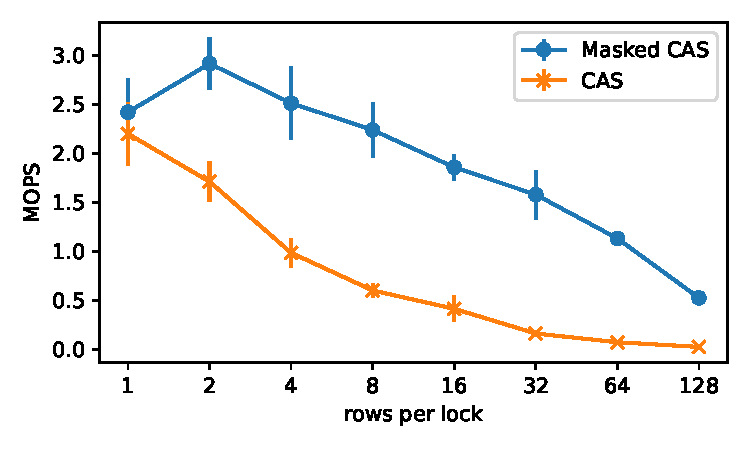
\includegraphics[width=0.99\linewidth]{fig/masked_cas_lock_size.pdf}
%    \end{subfigure}
    \begin{subfigure}{0.3\linewidth}
        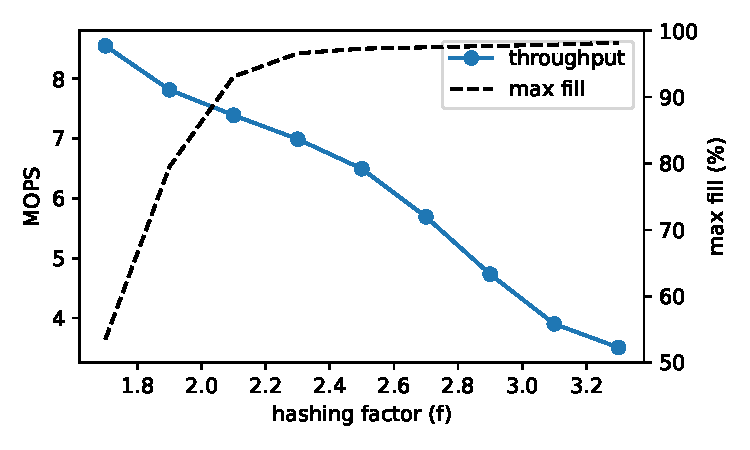
\includegraphics[width=0.99\linewidth]{fig/factor.pdf}
        % \label{fig:hash_fill}
        % \caption{}
    \end{subfigure}
    \begin{subfigure}{0.3\linewidth}
        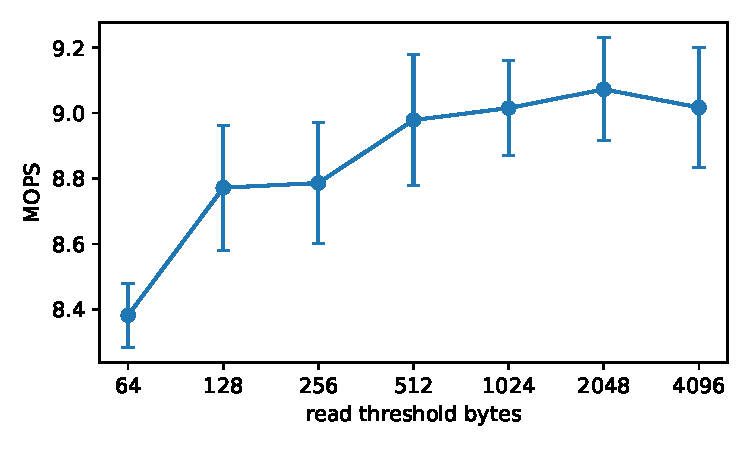
\includegraphics[width=0.99\linewidth]{fig/read_size.pdf}
        % \label{fig:hash_factor}
        % \caption{}
    \end{subfigure}
    %\begin{figure}[ht]
    \begin{subfigure}{0.3\linewidth}
      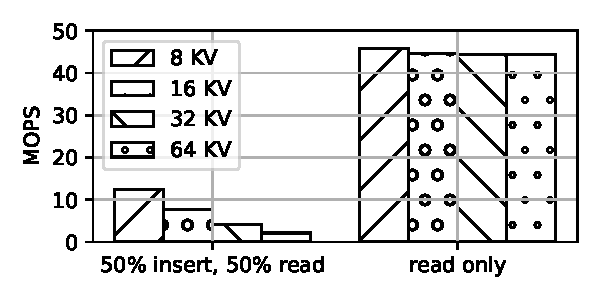
\includegraphics[width=0.99\linewidth]{fig/entry_size.pdf}
          \end{subfigure}
%    \caption{Throughput vs KV entry size}

%\end{figure}
    \vspace{-1em}
    \caption{RCuckoo parameter sweeps:
      \textbf{(a)} Throughput and max fill vs locality factor,
          \textbf{(b)} throughput vs read threshold, and 
    \textbf{(c)} throughput vs key/value entry size.
    }
    \label{fig:performance_breakdown}
             \label{fig:entry_size}
\end{figure*}

%% \subsubsection{Masked CAS}

%% Under contention masked CAS operations provide a significant
%% performance improvement. We measure it's benefit in terms of
%% throughput by comparing it with default CAS. In the
%% default case, when acquiring locks clients set the lock bits
%% for the locks they require and set all other bits in the cas
%% to 0. If the cas fails the current state of the lock table
%% over that range is returned as a result to the client and
%% the client tries to acquire their locks again using the
%% updated state of the lock table. Masked compare and swaps
%% are issued with the minimal mask required to set the locks.

%% Figure~\ref{fig:performance_breakdown} shows the improvement
%% gained by masked CAS. Default CAS operations perform better
%% with fewer rows per lock, as the probability of a lock being
%% set within the 64bit range is at its lowest. At higher rows
%% per lock CAS suffers from failed lock acquisitions from both
%% contested locks and due to a lack of synchronization. In
%% contrast masked CAS sees an improvement when two rows per
%% lock are used, as more second search attempts succeed, and
%% only suffers from direct lock contention as the rows per
%% lock increase.


\subsubsection{Parameter sweeps}

Figure~\ref{fig:performance_breakdown} plots the sensitivity of
RCuckoo performance to various parameter settings.

\textbf{Locality factor.}  The left-most graph shows that lower hash
factors $f$ deliver higher performance (plotted against the left axis)
due to better locality at the cost of lower expected maximum fill
factors (right axis).
%the tradeoff of their maximum fill factor. The
%relationship between $f$ and performance is nearly linear, while the
%relationship between $f$ and fill factor is
%exponential. Figure~\ref{fig:performance_breakdown}(c) shows the
%relationship between $f$, the max fill rate, and insert
%performance. These numbers were collected on an
This experiment consists of an insert-only workload (YCSB-W)
on a 100-M entry table. We choose an $f$ of 2.3 in practice as
it has the highest product of fill factor and throughput.
\todo{Section 4 says we use an f of 2.1?}

\textbf{Read threshold.}
\label{sec:read_threshold}
%As described in Section~\ref{sec:reading}
RCuckoo issues a covering
read if both key locations are within a defined threshold (128 bytes
in our experiments) of each other.
Figure~\ref{fig:performance_breakdown}(b) shows that performance
increases with larger thresholds, but at the cost of additional
bandwidth consumption.  In this experiment, only 40 clients
access a table with 64-byte rows, so they do not exhaust link bandwidth even with a 4-KB covering read, but performance levels off after 2 KB.
%% performance gains from increasing the read threshold. Here
%% each row is 64 bytes so our minimum threshold of 64 ensures
%% two packets are issued for each read request. We limit the
%% number of clients to 40 so that their is plenty of bandwidth
%% to support the inflated reads. Higher read thresholds trade
%% off network bandwidth for operation latency. 
Under these conditions, if bandwidth is plentiful larger (i.e., 2-KB
vs 128-B) covering reads can improve throughput, but only modestly.
%8\%.

% \begin{figure}[ht]
%     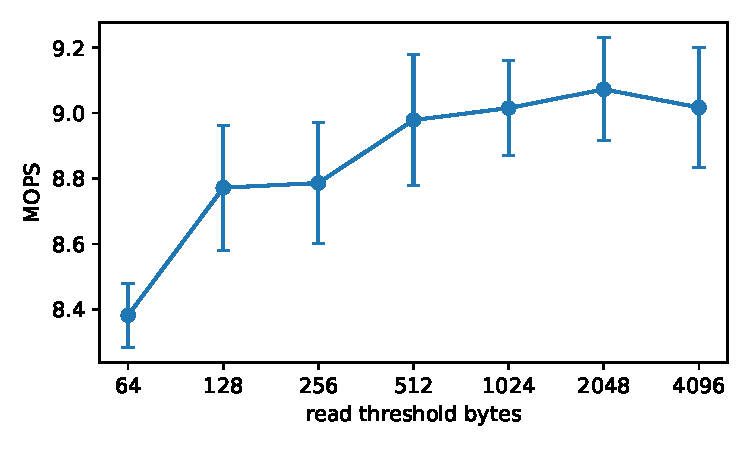
\includegraphics[width=0.99\linewidth]{fig/read_size.pdf}
%     \caption{Read Threshold vs Throughput}
%     \label{fig:read_threshold}
% \end{figure}


\textbf{Entry size.}  Inlined key/value entries enable RCuckoo's
single-round-trip reads, so the larger the entries, the fewer values
that require a second round trip.  However, for a fixed row size,
larger entries imply fewer entries per row, increasing cuckoo path
lengths (when measured in terms of rows), impacting insert performance.
%% but larger values must be stored in extents.  
%% at the cost of inflating the bandwidth of
%% operations. We run a 50\% read 50\% insert and a read only
%% workload to illustrate the overhead of larger entries.
Figure~\ref{fig:entry_size}(c) shows the effect of entry size on
operation throughput under YCSB-A. Insert is a bandwidth-limited
operation;
%quickly saturates
%the network bandwidth. At
at 16-B entries link capacity restricts throughput to 8 MOPS. The
performance of reads (and updates/deletes, not shown), on the other
hand, are largely unaffected by entry size.  Hence,
%which have lower
%bandwidth requirements see very little chance in throughput
%across entry sizes. We suggest that known read heavy
%workloads should use inlined entries as reads see a large
installations serving read-heavy workloads may wish to employ larger
entry sizes.
%
%boost in performance. Update operations are similarly
%unaffected by entry size up to 64 bytes. 

% Our design choice
% in embedding KV pairs is motivated by networking trends
% which suggest that 800 GBPS and higher network speeds will
% be available in the coming years. While round trip latency
% is expected to remain largely the same.




